\documentclass[a4paper,fleqn]{cas-dc}

\usepackage[numbers]{natbib}
\usepackage{amsmath,amssymb,amsfonts}
\usepackage{algorithmic}
\usepackage{algorithm}
\usepackage{textcomp}
\usepackage{xcolor}
\usepackage{booktabs}
\usepackage{multirow}
\usepackage{url}
\usepackage{subcaption}

\newcommand{\ecgr}{\textsf{ECGR}}
\newcommand{\cgr}{\textsf{CGR}}
\newcommand{\pecgr}{\textsf{P-ECGR}}

\begin{document}
\let\WriteBookmarks\relax
\def\floatpagepagefraction{1}
\def\textpagefraction{.001}

\shorttitle{Predictive Energy-Aware CGR for SmallSat Relays}
\shortauthors{J. Pandian and I. Kala}

\title [mode = title]{Predictive Energy-Aware Contact Graph Routing for SmallSat Relay Networks}

\author[1]{Jason Pandian}[
                        role=Researcher,
                        orcid=0000-0003-1702-5186,
                        bioid=1]
\cormark[1]
\ead{pandiajason@gmail.com}
\credit{Conceptualization, Methodology, Software, Formal analysis, Investigation, Data curation, Writing -- original draft, Visualization}

\affiliation[1]{organization={Department of Information Technology, Nehru Institute of Technology},
                city={Coimbatore}, 
                state={Tamil Nadu},
                country={India}}

\author[2]{I. Kala}[
                        role=Professor,
                        bioid=2]
\credit{Supervision, Validation, Writing -- review \& editing}

\affiliation[2]{organization={Department of Computer Science and Engineering, Nehru Institute of Technology},
                city={Coimbatore}, 
                state={Tamil Nadu},
                country={India}}

\cortext[cor1]{Corresponding author}

\begin{abstract}
Contact Graph Routing (CGR) is the de facto standard for store-carry-forward routing in deep-space Delay-Tolerant Networks (DTN). While CGR leverages the deterministic predictability of orbital contact schedules, it implicitly assumes that relay nodes possess sufficient energy and storage to execute all scheduled transmissions. This assumption breaks down in heterogeneous networks containing resource-constrained SmallSats, where standard CGR drains relay batteries to critical levels, causing packet drops. To address this, we propose two energy-aware routing strategies in this study: a baseline Energy-Aware CGR (\ecgr{}) that protects relay health based on instantaneous state metrics, and an improved Predictive Energy and Capacity-Aware Contact Graph Routing (\pecgr{}) that integrates a future energy prediction model and a reservation-based energy booking registry. By tracking committed transmissions, \pecgr{} prevents energy overbooking and load-balances traffic across heterogeneous relays. We evaluate both algorithms via discrete-event simulation of a Mars relay network using contact plans from synthetic SPICE ephemeris data. Over 10 Monte Carlo runs, both proposed algorithms maintain zero packet drops. The improved \pecgr{} achieves a bundle delivery ratio of $90.0 \pm 1.7\%$, outperforming standard CGR ($83.7 \pm 8.9\%$) and the proposed baseline \ecgr{} ($88.9 \pm 1.9\%$), while spending only $2.0 \pm 4.7\%$ of the time below $20\%$ battery SoC and significantly reducing delivery latency. The proposed algorithms add negligible computational overhead, making them suitable for flight-grade onboard processors.
\end{abstract}

\begin{graphicalabstract}
  \centering
  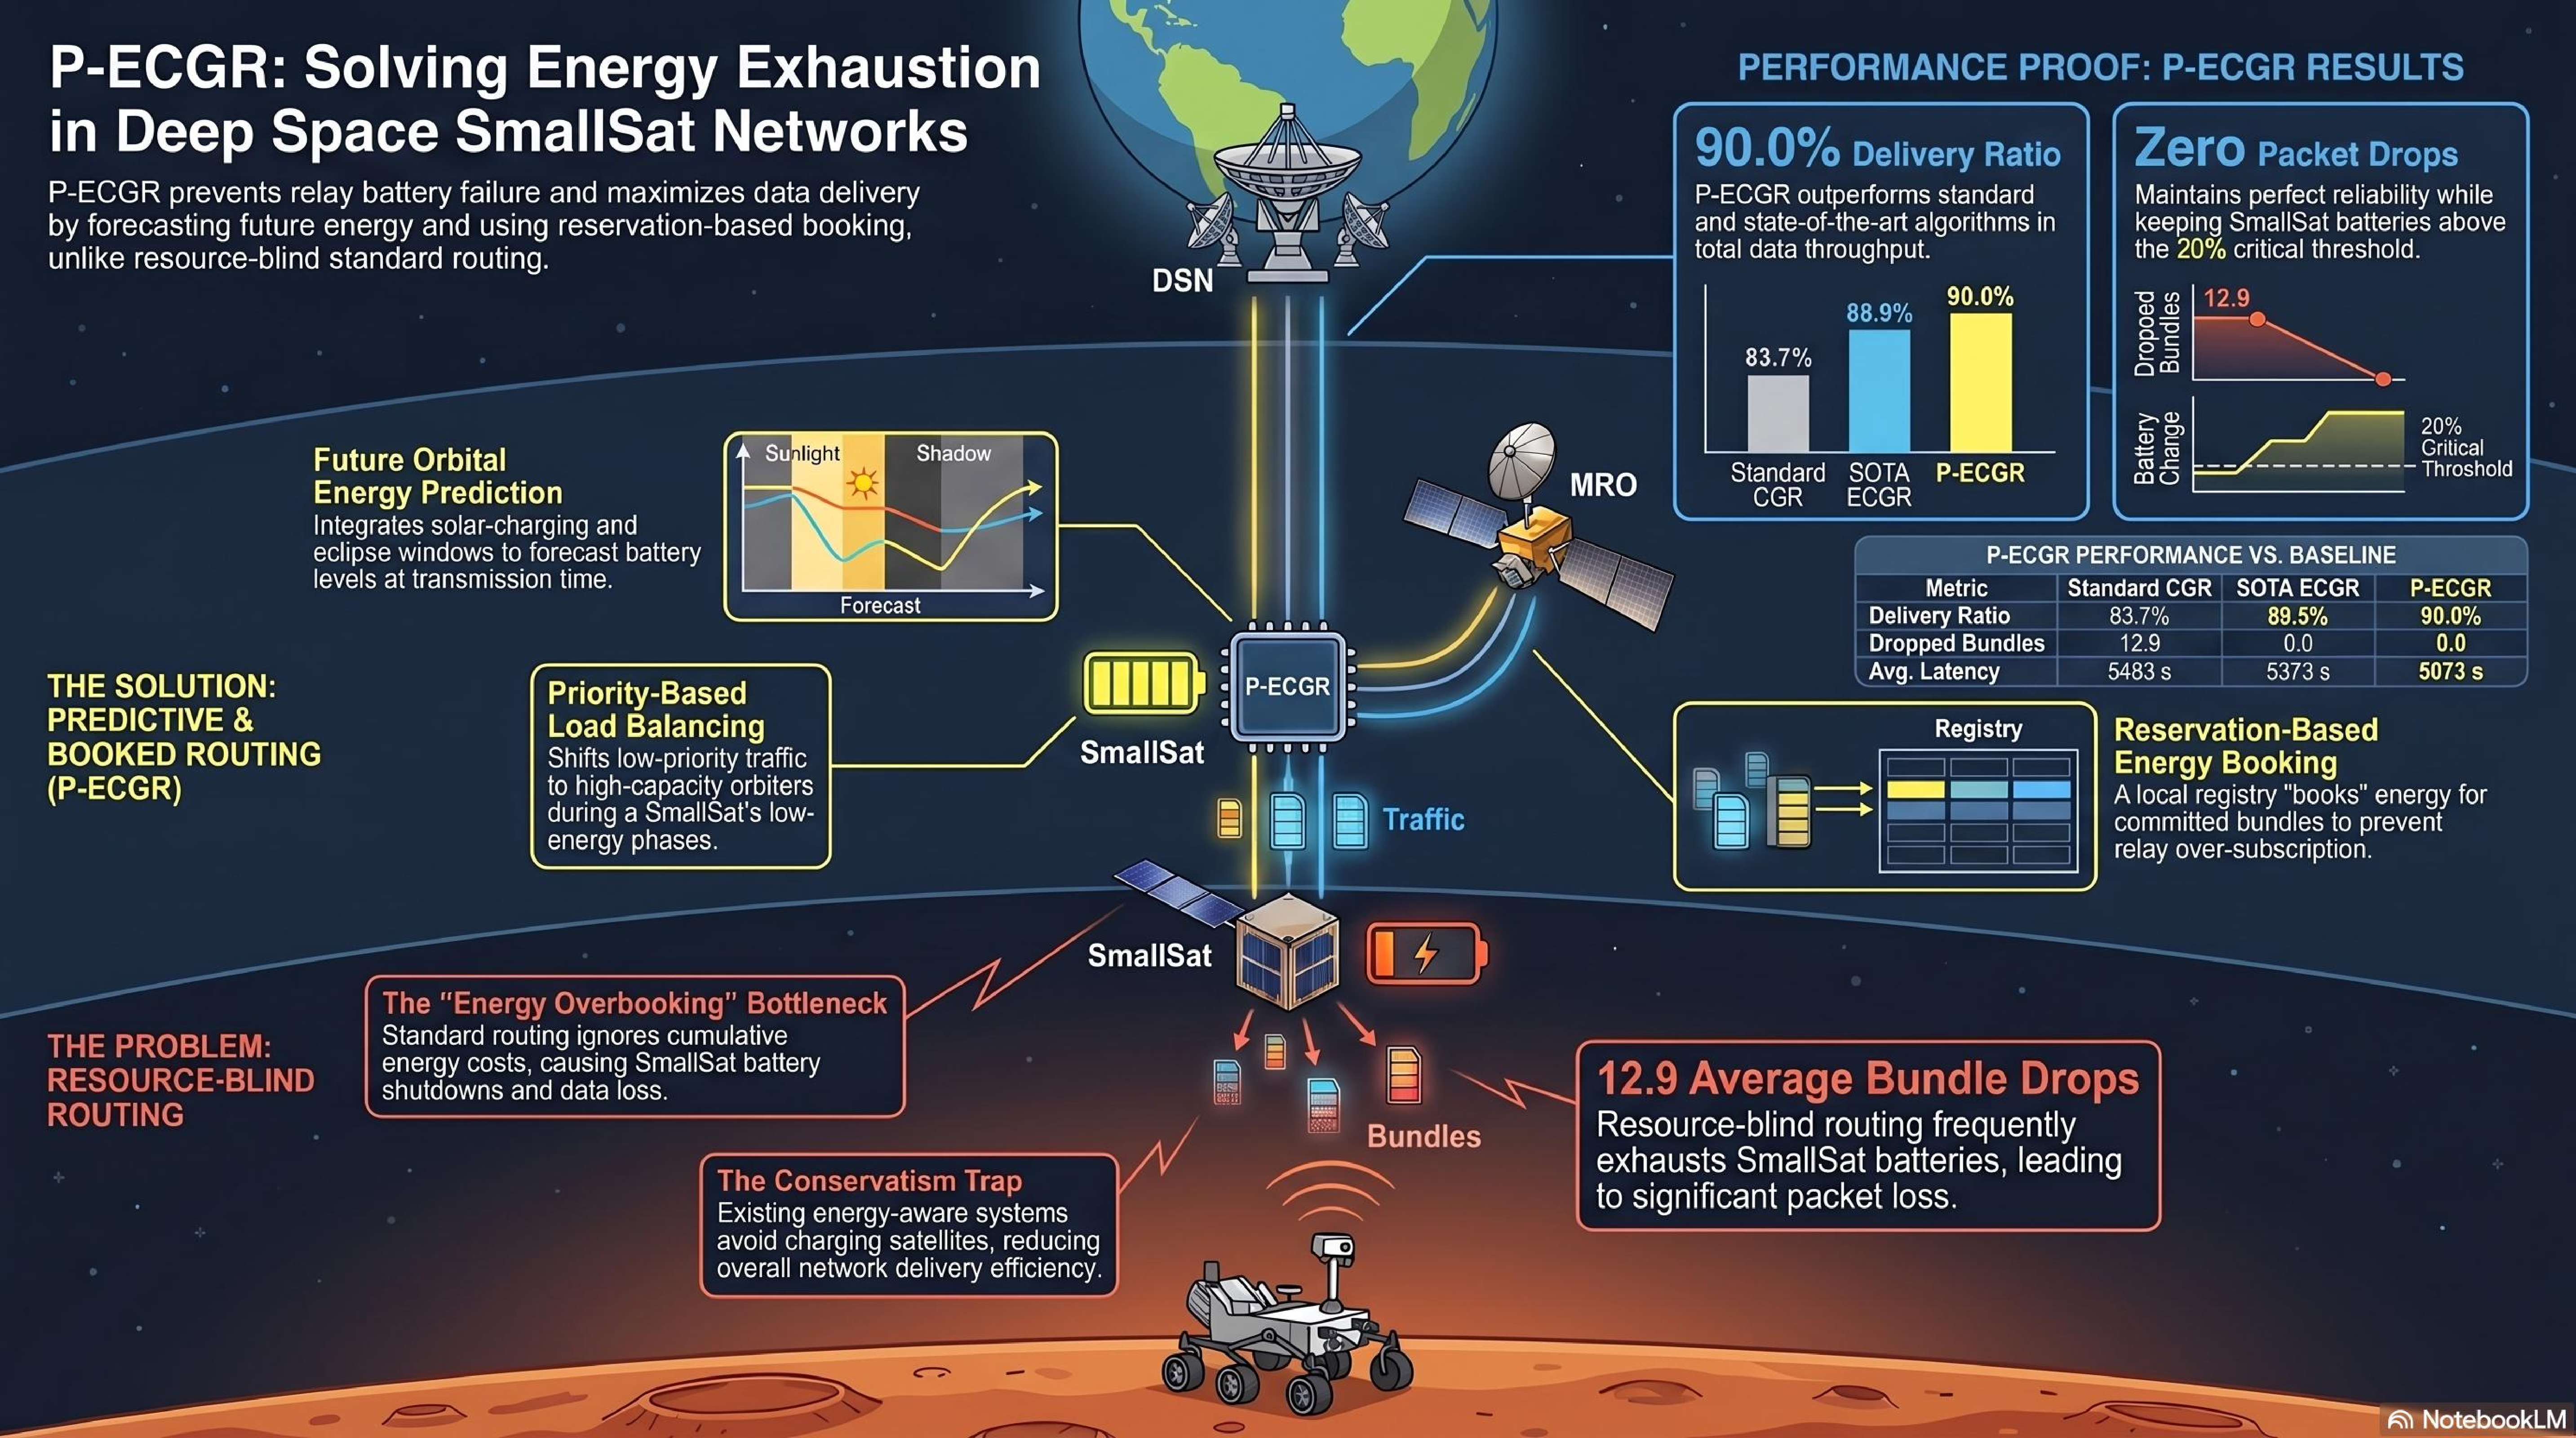
\includegraphics[width=\textwidth]{figs/P-ECGR_Deep_Space_Routing_Solution.png}
\end{graphicalabstract}

\begin{highlights}
  \item Presents Proposed ECGR and predictive P-ECGR routing for deep-space SmallSats.
  \item P-ECGR integrates solar-charging predictions with a discrete energy booking registry.
  \item Evaluates routing using a high-fidelity discrete-event planetary Mars relay simulator
  \item Both newly proposed algorithms eliminate bundle drops due to energy or buffer exhaustion
  \item Proposed predictive P-ECGR outperforms CGR \& ECGR in overall bundle delivery ratio.
\end{highlights}

\begin{keywords}
Delay-tolerant networking \sep Contact graph routing \sep Deep space communications \sep SmallSat \sep Energy-aware routing \sep Mars relay network
\end{keywords}

\maketitle

\section{Introduction}
\label{sec:intro}

\subsection{Deep Space Communication Bottlenecks}
Modern space exploration is transitioning from isolated, single-spacecraft missions to complex, multi-agent networks comprising rovers, landers, orbiters, and small satellite constellations. This paradigm shift requires high-bandwidth, reliable communication architectures. However, deep-space communications operate in environments characterized by extreme physical constraints, such as planetary occultations, orbital eclipses, massive free-space path losses over interplanetary distances, and solar plasma interference. 

Under these conditions, standard terrestrial network protocols, such as TCP/IP, fail catastrophically. TCP relies on continuous end-to-end paths and assumes that round-trip times (RTT) are short and packet loss is primarily caused by congestion. In contrast, deep-space links involve one-way light times (OWLT) ranging from several minutes to hours, and connectivity is highly intermittent due to orbital mechanics. To address these challenges, the Space Internet architecture leverages Delay-Tolerant Networking (DTN)~\cite{fall2003dtn,cerf2007dtn} and the Bundle Protocol version 7 (BPv7)~\cite{rfc9171}. DTN implements a store-carry-forward routing paradigm, where intermediate nodes store data in non-volatile memory buffers until a downstream communication opportunity (contact) becomes available.

\subsection{Store-Carry-Forward and CGR}
In space missions, the motion of celestial bodies and spacecraft is governed by orbital mechanics, rendering communication opportunities highly predictable. By utilizing ephemeris data, space agencies pre-compute a \emph{contact plan} that lists every scheduled communication window between nodes, including start times, durations, data rates, and propagation delays. 

Contact Graph Routing (CGR)~\cite{burleigh2010cgr} is the standard algorithm designed for these planned, scheduled-contact topologies. CGR represents the contact plan as a time-varying directed graph (the contact graph), where vertices represent communication contacts and edges denote time-ordered transitions between contacts. When a node needs to route a data packet (bundle), CGR runs a modified version of Dijkstra's algorithm to compute the path that minimizes end-to-end delivery delay (earliest arrival time). This approach is highly effective in homogeneous networks composed of well-provisioned spacecraft, such as NASA's Mars Reconnaissance Orbiter (MRO) or Mars Odyssey, which possess large solar arrays and high-capacity battery systems.

\subsection{Heterogeneous Space Networks and SmallSats}
The emergence of SmallSats and CubeSats (e.g., 3U and 6U form factors) has enabled low-cost, distributed missions, such as the MarCO CubeSats that tracked the InSight lander. Space agencies are planning to deploy swarms of SmallSats to provide localized relay coverage around Mars and the Moon~\cite{nasa2022artemis,yang2016smallsat}. However, these micro-platforms have extremely tight Size, Weight, and Power (SWaP) constraints. 

A typical 3U SmallSat relay possesses a small solar panel area, restricting average power generation to less than $10\,$W. Its battery capacity is restricted (e.g., $15$--$30\,$Wh), and its onboard buffer storage is limited (e.g., $256$--$512\,$MB). Crucially, operating a high-power radio transceiver during a transmission contact can consume $15$--$25\,$W, which is far greater than the average solar charging rate. As a result, active communication rapidly drains the satellite's battery. If the SmallSat is in Mars' shadow (orbital eclipse), it cannot generate solar power, and transmission must rely solely on the battery.

\subsection{Problem Statement}
Standard CGR is resource-blind. It assumes that if a contact window is listed in the contact plan, the transmitting node has sufficient electrical energy and storage capacity to complete the transfer. In a heterogeneous network consisting of a rover, a constrained SmallSat relay, a flagship orbiter, and Earth ground stations, CGR will route massive scientific images through the SmallSat relay simply because it offers the earliest contact window. This decision can deplete the SmallSat's battery, causing a low-voltage shutdown that drops all queued bundles and suspends housekeeping telemetry, jeopardizing the spacecraft's safety.

To protect relay node health, we propose a baseline Energy-Aware CGR (\ecgr{}) algorithm that evaluates node resource states during route computation. However, this proposed baseline \ecgr{} relies on \emph{instantaneous} battery state-of-charge (SoC) metrics at the routing epoch. This approach has two main limitations:
\begin{enumerate}
    \item \textbf{Resource Conservatism:} It penalizes routes through a node with a low battery state at $t_{\text{now}}$, even if that node will spend the next three hours in full sunlight charging its battery before the transmission contact actually begins. This conservatism reduces the delivery ratio and increases latency.
    \item \textbf{Energy Overbooking:} In multi-bundle scenarios, a source node processes bundles sequentially. If the source evaluates routes for twenty bundles in the same time step, each computation sees a safe instantaneous SoC at the relay. Consequently, the source routes all twenty bundles through the same SmallSat. The cumulative energy required to transmit this data far exceeds the SmallSat's battery capacity, causing battery exhaustion and packet drops.
\end{enumerate}

\subsection{Proposed Solution and Contributions}
To overcome these limitations, we propose an improved, predictive algorithm called \emph{Predictive Energy and Capacity-Aware Contact Graph Routing} (\pecgr{}). Both \ecgr{} and \pecgr{} are routing algorithms proposed in this work, with \pecgr{} representing a key prediction-based enhancement over the baseline \ecgr{}. Specifically, \pecgr{} integrates a future orbital solar-charging prediction model with a local reservation-based energy booking registry. The prediction model projects the relay's battery state forward to the start time of the future contact, taking into account predicted solar generation and eclipse periods. The energy-booking registry tracks committed transmissions, preventing energy overbooking. The contributions of this work are summarized as follows:
\begin{itemize}
    \item We identify and formulate the \emph{energy overbooking} bottleneck in resource-constrained routing for heterogeneous space networks.
    \item We propose a baseline \ecgr{} and an improved predictive \pecgr{} routing algorithm, incorporating future solar-charging predictions and a local energy booking registry to prevent energy overbooking and balance traffic load.
    \item We present a modular Python simulation framework that implements circular Keplerian orbit propagation, eclipse checks, and resource-constrained node models.
    \item We evaluate CGR, the proposed baseline \ecgr{}, and the proposed improved \pecgr{} on a Mars relay scenario, demonstrating that \pecgr{} achieves higher delivery ratios and lower latencies than baseline \ecgr{} while maintaining zero packet drops.
\end{itemize}

\subsection{Paper Outline}
The remainder of this paper is structured as follows. Section~\ref{sec:related} reviews related work in DTN and resource-aware routing. Section~\ref{sec:system} defines the system model, including topology, orbits, battery dynamics, and buffers. Section~\ref{sec:ecgr} details the routing formulations, presenting the algorithms for standard CGR, proposed baseline \ecgr{}, and proposed improved \pecgr{}. Section~\ref{sec:setup} describes the simulation setup and parameters. Section~\ref{sec:results} analyzes the results, and Section~\ref{sec:conclusion} concludes the paper.

% ====================================================================
\section{Related Work}
\label{sec:related}

\subsection{Delay-Tolerant Networking and Bundle Protocol}
The concept of Delay-Tolerant Networking originated from efforts to design an Interplanetary Internet, led by Cerf and others under the DARPA-funded Interplanetary Internet project. Fall~\cite{fall2003dtn} proposed a generalization of these concepts for challenged terrestrial and extraterrestrial environments, introducing the store-carry-forward routing paradigm. This architecture was formalized by the DTN Research Group (DTNRG) in RFC 4838~\cite{cerf2007dtn}. 

The Bundle Protocol (BP) serves as the primary protocol layer for DTN. BP resides between the application and transport/convergence layers, encapsulating application data into protocol data units called bundles. The protocol has evolved from version 6 (BPv6) to the modern version 7 (BPv7), which was standardized in RFC 9171~\cite{rfc9171} to support security and extensibility blocks. Satellite networking reviews, such as those by Caini et al.~\cite{caini2011dtn}, have demonstrated the benefits of BP in mitigating the effects of long round-trip times and frequent link disconnections in space communication links.

\subsection{Contact Graph Routing Advancements}
Contact Graph Routing was developed by Burleigh~\cite{burleigh2010cgr} to exploit the scheduled, predictable nature of space networks. Unlike routing protocols in terrestrial networks that rely on periodic route discovery packets, CGR utilizes pre-distributed contact plans. Fraire et al.~\cite{fraire2021cgr} provided a tutorial on CGR, detailing its Dijkstra-based path finding mechanics. 

Several enhancements have been proposed to improve CGR's performance. Araniti et al.~\cite{araniti2015contact} surveyed various routing strategies, including Space Active Bundle Routing (SABR) and opportunistic link integration. Segu{\'i} et al.~\cite{segui2011enhancing} adapted CGR for Mars relay operations planning, demonstrating the feasibility of using orbital schedules to route data from surface landers to Earth ground stations. However, these classical implementations assume that relay nodes have unlimited energy and memory buffers, an assumption that is invalid for SmallSat relays.

\subsection{Energy-Aware and Congestion-Aware Routing}
Congestion management in DTN space networks has been studied extensively. Madoery et al.~\cite{madoery2020congestion} proposed queue management and congestion-avoidance routing techniques to prevent buffer overflows at satellite relays. While these techniques protect storage buffers, they do not address battery limits.

Energy-constrained routing has received less attention in the context of CGR. Alessi et al.~\cite{alessi2019energy} proposed incorporating energy metrics into CGR, penalizing routes through nodes with low battery states. However, their formulation evaluated only the current, instantaneous battery SoC at the routing epoch. This approach leads to resource conservatism (avoiding nodes that will recharge before transmission) and fails to address the energy overbooking problem where multiple bundles are routed through the same node simultaneously. 

Machine learning and reinforcement learning approaches have been proposed for DTN routing (e.g., Dudukovich et al.~\cite{dudukovich2019dtn}). However, these algorithms require significant computational resources, making them unsuitable for radiation-hardened spacecraft processors, such as the RAD750 (operating at $133$--$200\,$MHz) or LEON3 processors, which have strict memory and CPU utilization limits. In contrast, our proposed \pecgr{} algorithm has low computational overhead and is backward-compatible with existing CGR systems.

% ====================================================================
\section{System Model}
\label{sec:system}

\subsection{Network Topology and Scenario}
We consider a four-node deep-space relay network modeling a realistic Mars exploration scenario, illustrated in Fig.~\ref{fig:topology}. The network consists of:
\begin{itemize}
    \item \textbf{Mars Surface Rover (Node 0):} Located at Jezero Crater ($4.5^\circ$S, $77.4^\circ$E). It acts as the primary data source, generating scientific images, critical telemetry, and housekeeping data. The rover is powered by a Multi-Mission Radioisotope Thermoelectric Generator (MMRTG) providing constant power generation.
    \item \textbf{SmallSat Relay (Node 1):} A resource-constrained 3U CubeSat in a near-polar Sun-synchronous circular orbit. It has a small battery, constrained buffer, and is solar-powered, meaning its power generation is zero during eclipses.
    \item \textbf{Mars Reconnaissance Orbiter (Node 2):} A flagship-class orbiter in low Mars orbit. It possesses a high-capacity battery, large solar arrays, and a large storage buffer, allowing it to act as a high-capacity relay.
    \item \textbf{Deep Space Network (Node 3):} Earth ground stations, representing the destination. The DSN has effectively unlimited energy, buffer capacity, and processing power.
\end{itemize}

\begin{figure}[t]
    \centering
    
\includegraphics[width=\columnwidth]{figs/fig8_topology.pdf}
    \caption{Mars relay network topology showing the four-node scenario with link types and data rates. The SmallSat relay (Node~1) is the resource-constrained bottleneck.}
    \label{fig:topology}
\end{figure}

\subsection{Orbits and Visibility Model}
The positions of the SmallSat relay and MRO are propagated using Keplerian circular orbits around Mars. The orbital radius $r$ is defined as:
\begin{equation}
    r = R_M + h
\end{equation}
where $R_M = 3389.5\,$km is the mean radius of Mars, and $h$ is the altitude of the satellite ($400\,$km for SmallSat, $300\,$km for MRO). The orbital period $T$ is computed using Kepler's third law:
\begin{equation}
    T = 2\pi \sqrt{\frac{r^3}{GM_M}}
\end{equation}
where $GM_M = 4.282837 \times 10^{13}\,\text{m}^3/\text{s}^2$ is the gravitational parameter of Mars. This yields an orbital period of approximately $7{,}560\,$s ($2.1\,$h) for the SmallSat and $6{,}840\,$s ($1.9\,$h) for the MRO.

A communication link between a surface node (rover) and an orbiter is feasible only when the orbiter is above the rover's local horizon. Geometrically, the elevation angle $\theta_{el}$ of the satellite relative to the rover must exceed a minimum elevation mask $\theta_{mask} = 10^\circ$ to clear topography and minimize atmospheric attenuation. The line-of-sight vector $\mathbf{d}$ from the rover position $\mathbf{p}_r$ to the satellite position $\mathbf{p}_s$ is:
\begin{equation}
    \mathbf{d} = \mathbf{p}_s - \mathbf{p}_r
\end{equation}
The elevation angle is defined as:
\begin{equation}
    \theta_{el} = 90^\circ - \arccos\left(\frac{\mathbf{d} \cdot \mathbf{p}_r}{\|\mathbf{d}\| \|\mathbf{p}_r\|}\right)
\end{equation}
A contact is created when $\theta_{el} \geq \theta_{mask}$ and the line of sight is not obstructed by Mars.

\subsection{Energy Model}
For each non-ground node, the battery energy state $E(t)$ (Wh) is modeled as a continuous state-of-charge equation:
\begin{equation}
    E(t + \Delta t) = \min\left(E_{\max},\; \max\left(0,\; E(t) + \Delta E_{\text{net}}\right)\right)
\end{equation}
where $E_{\max}$ is the battery capacity, and $\Delta E_{\text{net}}$ is the net energy change over time step $\Delta t$, computed as:
\begin{equation}
    \Delta E_{\text{net}} = \left(P_{\text{gen}}(t) - P_{\text{cons}}(t)\right) \cdot \frac{\Delta t}{3600} \quad \text{[Wh]}
\end{equation}
The power generation $P_{\text{gen}}(t)$ depends on whether the node is in Mars' shadow:
\begin{equation}
    P_{\text{gen}}(t) = \begin{cases}
        0.0 & \text{if in eclipse} \\
        P_{\text{solar}} & \text{otherwise}
    \end{cases}
\end{equation}
Eclipses occur when Mars obstructs the line of sight between the satellite and the Sun. The power consumption $P_{\text{cons}}(t)$ is:
\begin{equation}
    P_{\text{cons}}(t) = P_{\text{idle}} + P_{\text{tx}} \cdot \mathbb{1}_{\text{tx}}(t) + P_{\text{rx}} \cdot \mathbb{1}_{\text{rx}}(t)
\end{equation}
where $P_{\text{idle}} $ is the baseline system power, $P_{\text{tx}} $ is the additional power consumed by the radio transmitter during active transmission, $P_{\text{rx}} $ is the power consumed by the receiver during active reception, and $\mathbb{1}_{\text{tx}}, \mathbb{1}_{\text{rx}} \in \{0, 1\}$ are indicators of transmission and reception activity.

The state of charge (SoC) is defined as:
\begin{equation}
    \text{SoC}(t) = \frac{E(t)}{E_{\max}}
\end{equation}
If the battery SoC drops to $0.0$, the node shuts down, dropping all bundles currently stored in its buffer.

\subsection{Buffer Model}
Each node $n$ has a physical buffer storage capacity $B_{\max}^n$ bytes. The buffer utilization $U_B(t)$ is the fraction of capacity occupied by queued bundles:
\begin{equation}
    U_B(t) = \frac{\sum_{b \in \mathcal{Q}(t)} |b|}{B_{\max}^n}
\end{equation}
where $\mathcal{Q}(t)$ is the set of bundles stored in node $n$'s queue at time $t$, and $|b|$ is the size of bundle $b$ in bytes. The available buffer space is:
\begin{equation}
    B_{\text{avail}}^n(t) = B_{\max}^n - \sum_{b \in \mathcal{Q}(t)} |b|
\end{equation}
If a node receives a bundle $b$ when $B_{\text{avail}}^n < |b|$, the bundle is dropped due to buffer overflow.

\subsection{Traffic Generation Model}
The rover generates three classes of traffic, characterized by priority, bundle size, and arrival intervals:
\begin{enumerate}
    \item \textbf{Priority 1 (Critical Telemetry):} Consists of small health and status reports (size range $1.0$--$5.0\,$MB) generated at short intervals ($1000$--$2000\,$s). These bundles require low latency.
    \item \textbf{Priority 2 (Scientific Images):} Consists of large scientific files (size range $15.0$--$90.0\,$MB) generated at longer intervals ($2000$--$4000\,$s). These bundles represent the bulk of the network volume.
    \item \textbf{Priority 3 (Housekeeping Data):} Consists of small, routine reports (size range $0.2$--$2.0\,$MB) generated at short intervals ($500$--$1000\,$s). These have the lowest priority.
\end{enumerate}

% ====================================================================
\section{Routing Algorithms and Formulations}
\label{sec:ecgr}

In this section, we present the formulations of the three routing algorithms evaluated in this study: standard Contact Graph Routing (CGR), our proposed baseline Energy-Aware CGR (ECGR), and our proposed Predictive Energy and Capacity-Aware CGR (P-ECGR). Both ECGR and P-ECGR are developed in this work, with P-ECGR serving as an improved, prediction-based extension of the baseline ECGR.

\subsection{Standard Contact Graph Routing (CGR)}
Standard CGR aims to minimize delivery delay. Given a bundle $b$ created at time $t_{\text{now}}$, CGR identifies all feasible routes to the destination. For each route $r$, composed of a sequence of contacts $r = (c_1, c_2, \dots, c_k)$, the arrival time $T_{\text{arr}}(r)$ is:
\begin{equation}
    T_{\text{arr}}(r) = t_{\text{end}}(c_k) + \tau_{\text{owlt}}(c_k)
\end{equation}
CGR filters out routes that violate link capacities or create routing loops. A route $r$ is feasible if:
\begin{equation}
    C_{\text{resid}}(c_i) \geq |b| \quad \forall c_i \in r
\end{equation}
where $C_{\text{resid}}(c_i)$ is the residual capacity of contact $c_i$. The optimal route $r^*$ is selected to minimize arrival time:
\begin{equation}
    r^* = \arg\min_{r \in \mathcal{R}_f} T_{\text{arr}}(r)
\end{equation}
where $\mathcal{R}_f$ is the set of capacity-feasible routes. CGR is resource-blind: it does not evaluate whether the nodes along the route have the energy to complete the transmissions.

\subsection{Proposed Baseline Energy-Aware CGR (ECGR)}
The proposed baseline \ecgr{} incorporates relay battery and buffer states into a multi-attribute cost function:
\begin{equation}
    \mathcal{C}_{\text{ECGR}}(r, b) = \alpha \cdot \hat{D}(r) + \beta \cdot \Phi_E(r) + \gamma \cdot \Phi_B(r, b)
\end{equation}
where:
\begin{itemize}
    \item $\hat{D}(r) = D(r) / D_{\max}$ is the normalized route delay, with $D(r) = T_{\text{arr}}(r) - t_{\text{now}}$ and $D_{\max} = \max_{r' \in \mathcal{R}_f} D(r')$.
    \item $\Phi_E(r) = 1.0 / \min_{n \in \mathcal{R}(r)} \text{SoC}_n(t_{\text{now}})$ is the energy penalty, which is inversely proportional to the minimum instantaneous SoC among the relay nodes $\mathcal{R}(r)$.
    \item $\Phi_B(r, b) = \max_{n \in \mathcal{R}(r)} (|b| / B_{\text{avail}}^n(t_{\text{now}}))$ is the buffer penalty, reflecting the fraction of available storage the bundle would occupy.
    \item $\alpha, \beta, \gamma$ are dynamic weights scaled based on bundle priority and instantaneous warning/critical thresholds.
\end{itemize}

During route selection, baseline \ecgr{} filters out routes if any relay node cannot transmit the bundle based on its current energy state:
\begin{equation}
    E_n(t_{\text{now}}) < (P_{\text{tx}}^n + P_{\text{idle}}^n) \cdot \frac{8 \cdot |b|}{R_{\text{link}}} \cdot \frac{1}{3600}
\end{equation}
The proposed baseline \ecgr{} route-selection procedure is detailed in Algorithm~\ref{alg:sota_ecgr}.

\begin{algorithm}[h]
\caption{Proposed Baseline \ecgr{} Route Selection}
\label{alg:sota_ecgr}
\begin{algorithmic}[1]
\REQUIRE Contact plan $\mathcal{C}$, bundle $b$, node states $\mathcal{N}$, current time $t_{\text{now}}$
\ENSURE Selected route $r^*$ or $\emptyset$
\STATE $\mathcal{R} \leftarrow$ \textsc{FindAllRoutes}($\mathcal{C}$, $b.\text{src}$, $b.\text{dst}$, $t_{\text{now}}$)
\STATE $\mathcal{R}_f \leftarrow \emptyset$
\FOR{each $r \in \mathcal{R}$}
    \STATE $capacity\_ok \leftarrow \text{True}$
    \FOR{each hop $h \in r.\text{hops}$}
        \IF{$h.\text{residual\_capacity} < b.\text{size\_bytes}$}
            \STATE $capacity\_ok \leftarrow \text{False}$
        \ENDIF
    \ENDFOR
    \IF{\NOT $capacity\_ok$}
        \STATE \textbf{continue}
    \ENDIF
    \STATE $relay\_ok \leftarrow \text{True}$
    \FOR{each relay node $n \in r.\text{relay\_nodes}$}
        \STATE $tx\_time \leftarrow b.\text{size\_bytes} \cdot 8 / r.\text{bottleneck\_rate}$
        \IF{\NOT $\mathcal{N}[n].\text{can\_store}(b.\text{size\_bytes})$ \OR \NOT $\mathcal{N}[n].\text{can\_transmit}(tx\_time)$}
            \STATE $relay\_ok \leftarrow \text{False}$
        \ENDIF
    \ENDFOR
    \IF{$relay\_ok$}
        \STATE $\mathcal{R}_f \leftarrow \mathcal{R}_f \cup \{r\}$
    \ENDIF
\ENDFOR
\IF{$\mathcal{R}_f = \emptyset$}
    \RETURN $\emptyset$
\ENDIF
\STATE $D_{\max} \leftarrow \max_{r \in \mathcal{R}_f} D(r)$
\STATE Selected route $r^* \leftarrow \arg\min_{r \in \mathcal{R}_f} \mathcal{C}_{\text{ECGR}}(r, b; \mathcal{N}, D_{\max}, t_{\text{now}})$
\RETURN $r^*$
\end{algorithmic}
\end{algorithm}

\subsection{Proposed Predictive and Energy-Booked ECGR (P-ECGR)}
Proposed \pecgr{} replaces the instantaneous metrics of the proposed baseline \ecgr{} with a predictive orbital energy model and a local energy booking registry to resolve the energy overbooking problem.

\subsubsection{Future Energy Prediction Model}
Instead of evaluating the instantaneous energy state $E_n(t_{\text{now}})$, \pecgr{} predicts the battery energy state $E_{\text{pred}}(n, t_{\text{start}})$ at the future start time $t_{\text{start}}$ of the contact window. The prediction is computed by integrating the nominal solar generation and idle drain rates over the propagation delay:
\begin{equation}
    E_{\text{pred}}(n, t_{\text{start}}) = E_n(t_{\text{now}}) + \int_{t_{\text{now}}}^{t_{\text{start}}} \left( P_{\text{gen}}(n, t) - P_{\text{idle}}(n) \right) dt
\end{equation}
where $P_{\text{gen}}(n, t)$ is modeled as $P_{\text{solar}}^n \cdot (1 - \text{shadow}(n, t))$, and $\text{shadow}(n, t) \in \{0, 1\}$ is a step function derived from predicted orbital eclipse windows. The predicted energy is bounded by the battery capacity $E_{\max}^n$:
\begin{equation}
    0 \leq E_{\text{pred}}(n, t_{\text{start}}) \leq E_{\max}^n
\end{equation}

\subsubsection{Energy-Booking Reservation Registry}
To prevent energy overbooking, \pecgr{} maintains a local reservation registry $\mathcal{R}_{\text{book}}$. When a route $r$ is selected for bundle $b$, the expected transmission energy $E_{\text{tx}}(b)$ is computed as:
\begin{equation}
    E_{\text{tx}}(b) = \left( P_{\text{tx}}(n) + P_{\text{idle}}(n) \right) \cdot \frac{8 \cdot |b|}{R_{\text{link}}} \cdot \frac{1}{3600} \quad \text{[Wh]}
\end{equation}
This energy consumption is booked in the registry for node $n$ at the contact's start time $t_{\text{start}}$.

When evaluating subsequent bundles, the net predicted energy $E_{\text{net}}(n, t_{\text{start}})$ is computed by subtracting all booked energy allocations scheduled to transmit prior to $t_{\text{start}}$:
\begin{equation}
    E_{\text{net}}(n, t_{\text{start}}) = E_{\text{pred}}(n, t_{\text{start}}) - \sum_{k \in \mathcal{K}_n(t_{\text{now}}, t_{\text{start}})} E_{\text{tx}}(b_k)
\end{equation}
where $\mathcal{K}_n(t_{\text{now}}, t_{\text{start}})$ is the set of bundle IDs booked for transmission on node $n$ during the interval $[t_{\text{now}}, t_{\text{start}})$. Registry entries scheduled in the past ($t < t_{\text{now}}$) are pruned, as their actual energy drain is already reflected in the node's real-time state $E_n(t_{\text{now}})$.

\subsubsection{Energy Penalty Deadband Function}
Let the predicted state of charge be $\text{SoC}_{\text{pred}}(n) = E_{\text{net}}(n, t_{\text{start}}) / E_{\max}^n$. The predicted post-transmission SoC after sending bundle $b$ is:
\begin{equation}
    \text{SoC}_{\text{post}}(n) = \text{SoC}_{\text{pred}}(n) - \frac{E_{\text{tx}}(b)}{E_{\max}^n}
\end{equation}
To avoid penalizing routes when the relay operates in the safe energy zone, we implement a deadband penalty function $\Phi_E(r, b) = \sum_{n \in \mathcal{R}(r)} \phi_E(n, b)$, where:
\begin{equation}
    \phi_E(n, b) = \begin{cases}
        0.0 & \text{SoC}_{\text{post}}(n) \geq \theta_{\text{warn}} \\
        \lambda \cdot \frac{\theta_{\text{warn}} - \text{SoC}_{\text{post}}(n)}{\theta_{\text{warn}}} & \theta_{\text{crit}} \leq \text{SoC}_{\text{post}}(n) < \theta_{\text{warn}} \\
        \Omega & \text{SoC}_{\text{post}}(n) < \theta_{\text{crit}}
    \end{cases}
\end{equation}
where $\theta_{\text{warn}} = 0.35$ and $\theta_{\text{crit}} = 0.20$ are the warning and critical battery thresholds, $\lambda = 10.0$ is the warning scale factor, and $\Omega = 50.0$ is the severe critical penalty.

\subsubsection{Priority-Based Weight Adaptation}
The weights $(\alpha, \beta, \gamma)$ scale adaptively to balance delay minimization with resource protection. First, the base weights $(\alpha_0, \beta_0, \gamma_0)_p$ are determined by the bundle's priority class $p$:
\begin{equation}
    (\alpha_0, \beta_0, \gamma_0)_p = \begin{cases}
        (2.0, 0.5, 0.5) & p = 1 \text{ (Critical)} \\
        (1.0, 1.0, 1.0) & p = 2 \text{ (Normal)} \\
        (0.3, 2.0, 2.0) & p = 3 \text{ (Low)}
    \end{cases}
\end{equation}
Second, the weights are scaled dynamically according to the net predicted energy state:
\begin{equation}
    \beta' = \beta_0 \cdot \begin{cases}
        4.0 & \text{if } E_{\text{net}} < \theta_{\text{crit}} \cdot E_{\max} \\
        2.0 & \text{if } \theta_{\text{crit}} \cdot E_{\max} \leq E_{\text{net}} < \theta_{\text{warn}} \cdot E_{\max} \\
        1.0 & \text{otherwise}
    \end{cases}
\end{equation}
\begin{equation}
    \gamma' = \gamma_0 \cdot \begin{cases}
        3.0 & \text{if } U_B^{\max} > 0.70 \\
        1.0 & \text{otherwise}
    \end{cases}
\end{equation}

\subsubsection{Feasibility Filtering}
Before cost calculation, candidate routes are filtered for feasibility. A route $r$ is feasible for bundle $b$ if and only if:
\begin{enumerate}
    \item The residual capacity of each contact hop exceeds $|b|$:
    \begin{equation}
        C_{\text{resid}}(c) \geq |b| \quad \forall c \in r
    \end{equation}
    \item The available buffer at each relay node exceeds $|b|$:
    \begin{equation}
        B_{\text{avail}}^n \geq |b| \quad \forall n \in \mathcal{R}(r)
    \end{equation}
    \item The net predicted energy at transmission start time exceeds the energy required for transmission:
    \begin{equation}
        E_{\text{net}}(n, t_{\text{start}}) \geq E_{\text{tx}}(b) \quad \forall n \in \mathcal{R}(r)
    \end{equation}
\end{enumerate}

The complete \pecgr{} route-selection procedure is detailed in Algorithm~\ref{alg:pecgr}.

\begin{algorithm}[t]
\caption{\pecgr{} Route Selection and Energy Booking}
\label{alg:pecgr}
\begin{algorithmic}[1]
\REQUIRE Contact plan $\mathcal{C}$, bundle $b$, node states $\mathcal{N}$, local booking registry $\mathcal{R}_{\text{book}}$, time $t$
\ENSURE Selected route $r^*$ or $\emptyset$
\STATE $\mathcal{R} \leftarrow$ \textsc{FindAllRoutes}($\mathcal{C}$, $b.\text{src}$, $b.\text{dst}$, $t$)
\STATE $\mathcal{R}_f \leftarrow \emptyset$
\STATE \textsc{CleanExpiredBookings}($\mathcal{R}_{\text{book}}$, $t$)
\STATE \textsc{RemovePriorReservations}($\mathcal{R}_{\text{book}}$, $b.\text{id}$)
\FOR{each $r \in \mathcal{R}$}
    \IF{\textsc{CheckLinkCapacity}($r$, $b$) \AND \textsc{CheckBufferSpace}($r$, $b$, $\mathcal{N}$) \AND \textsc{CheckPredictiveEnergy}($r$, $b$, $\mathcal{N}$, $\mathcal{R}_{\text{book}}$, $t$)}
        \STATE $\mathcal{R}_f \leftarrow \mathcal{R}_f \cup \{r\}$
        \STATE Compute predicted SoCs for $r$ using $E_{\text{net}}(n, t_{\text{start}})$
    \ENDIF
\ENDFOR
\IF{$\mathcal{R}_f = \emptyset$}
    \RETURN $\emptyset$
\ENDIF
\STATE $D_{\max} \leftarrow \max_{r \in \mathcal{R}_f} D(r)$
\STATE $(\alpha, \beta, \gamma) \leftarrow$ \textsc{GetAdaptiveWeights}($b$, $\mathcal{N}$, $\mathcal{R}_{\text{book}}$, $t$)
\STATE $r^* \leftarrow \arg\min_{r \in \mathcal{R}_f} \mathcal{C}(r, b; \alpha, \beta, \gamma, D_{\max})$
\IF{$r^* \neq \emptyset$}
    \FOR{each hop $h \in r^*$ with source node $n \in \mathcal{R}(r^*)$}
        \STATE $E_{\text{tx}} \leftarrow$ \textsc{ComputeTxEnergy}($n$, $b$, $h.\text{rate}$)
        \STATE \textsc{RegisterBooking}($\mathcal{R}_{\text{book}}$, $n$, $h.\text{start\_time}$, $E_{\text{tx}}$, $b.\text{id}$)
    \ENDFOR
\ENDIF
\RETURN $r^*$
\end{algorithmic}
\end{algorithm}

% ====================================================================
\section{Python Simulation Setup}
\label{sec:setup}

To evaluate the performance of standard CGR, the proposed baseline \ecgr{}, and the proposed improved \pecgr{}, we developed a discrete-time event-driven Python simulator representing the deep-space Mars relay scenario.

\subsection{Simulator Package Structure}
The simulator codebase is structured as a modular package containing the following core files:
\begin{itemize}
    \item \textsf{config.py:} Defines all global parameters, including simulation duration ($86{,}400\,$s), time step size ($10\,$s), node SWaP specs (Table~\ref{tab:params}), link parameters, and priority weights.
    \item \textsf{models.py:} Implements the data models for `Contact`, `Bundle`, `Node`, and `Route`. The `Node` class encapsulates energy update equations, battery charging/discharging logic, and buffer storage checks.
    \item \textsf{spice\_data.py:} Implements the synthetic SPICE ephemeris engine, generating Keplerian orbital trajectories for the SmallSat relay and MRO around Mars and checking for eclipses and line-of-sight visibility windows.
    \item \textsf{contact\_plan.py:} Generates contact plans based on the visibility calculations and exports them to JSON and standard JPL ION-DTN configuration format.
    \item \textsf{routing.py:} Implements the routing decision logic for `CGRRouter`, `ECGRRouter`, and `EBECGRRouter` (P-ECGR).
    \item \textsf{simulator.py:} Implements the main discrete-event execution loop. In each step, the simulator updates node batteries, injects newly generated bundles, and evaluates route options for queued bundles.
\end{itemize}

\subsection{Synthetic SPICE and Orbital Generation}
The simulator generates orbital trajectories utilizing circular Keplerian motion. The position vector $\mathbf{r}(t)$ of a satellite in orbit is represented as:
\begin{equation}
    \mathbf{r}(t) = r \cos(\omega t) \mathbf{\hat{u}} + r \sin(\omega t) \mathbf{\hat{v}}
\end{equation}
where $r$ is the orbital radius, $\omega = 2\pi / T$ is the angular velocity, and $\mathbf{\hat{u}}, \mathbf{\hat{v}}$ are orthogonal unit vectors defining the orbital plane. The inclination angles are set to $87^\circ$ for the SmallSat relay and $93^\circ$ for the MRO, representing typical polar science orbits. Eclipses are modeled using a cylindrical projection of Mars' shadow. A satellite is in eclipse if:
\begin{equation}
    \mathbf{r}(t) \cdot \mathbf{\hat{s}} < 0 \quad \text{and} \quad \|\mathbf{r}(t) - (\mathbf{r}(t) \cdot \mathbf{\hat{s}})\mathbf{\hat{s}}\| < R_M
\end{equation}
where $\mathbf{\hat{s}}$ is the unit vector pointing toward the Sun.

\subsection{Simulation Scenario and Traffic Loading}
The simulation models a $24$-hour Martian day. The rover (Node 0) generates data according to the three profiles described in Section~\ref{sec:system}. A total of $199$ bundles are generated over the day, representing approximately $2.1\,$GB of scientific and telemetry data. The SmallSat relay (Node 1) and MRO (Node 2) act as relays to deliver these bundles to the DSN (Node 3) on Earth. 

The link from MRO to DSN has a data rate of $2\,$Mbps, and MRO is well-provisioned (battery capacity $1120\,$Wh, solar power $1000\,$W). In contrast, the link from the SmallSat relay to DSN is slower ($500\,$kbps), and the SmallSat is highly constrained (battery capacity $16\,$Wh, solar power $8\,$W, transmission power draw $15\,$W). This configuration creates a resource bottleneck at the SmallSat relay, testing the resource-awareness of the routing algorithms.

\subsection{Simulation Parameters}
The simulation parameters are summarized in Table~\ref{tab:params}.

\begin{table}[t]
\centering
\caption{Simulation Parameters}
\label{tab:params}
\begin{tabular}{ll}
\hline
\textbf{Parameter} & \textbf{Value} \\
\hline
Simulation Duration & 86,400 s (24.0 h) \\
SmallSat Battery & 16.0 Wh \\
SmallSat Solar Power & 8.0 W (avg) \\
SmallSat Buffer & 512 MB \\
SmallSat Tx Power & 15.0 W \\
MRO Battery & 1120.0 Wh \\
MRO Buffer & 8192 MB \\
Rover-SmallSat Rate & 2 Mbps (UHF) \\
MRO-DSN Rate & 2 Mbps (X-band) \\
Earth-Mars OWLT & ~750 s \\
Monte Carlo Runs & 10 \\
\hline
\end{tabular}
\end{table}

\subsection{Monte Carlo Configuration}
To obtain statistically significant results, we execute $10$ independent Monte Carlo runs. The orbital contact plan is kept identical across all runs (since orbits are deterministic), but the traffic generation seeds are varied deterministically as $42 + 17i$ for run $i$. This approach introduces variance in bundle creation times, sizes, and priority sequences.

\subsection{Performance Evaluation Metrics}
\label{sec:metrics}
To quantify the behavior of the three routing schemes (\cgr{}, \ecgr{}, and \pecgr{}) we collect a set of complementary metrics that capture throughput, latency, reliability, and resource usage of the SmallSat relay. All metrics are computed over the 10 Monte‑Carlo simulation runs and reported as mean $\pm$ one standard deviation.
\begin{itemize}
  \item \textbf{Bundle Delivery Ratio (BDR)} (\%):
        \begin{equation}
          \text{BDR}
          = \frac{N_{\text{delivered}}}{N_{\text{generated}}}\times 100,
        \end{equation}
        where $N_{\text{generated}}$ is the total number of bundles injected into the network and $N_{\text{delivered}}$ is the number that reach the destination before the 24‑hour simulation deadline. BDR directly measures the effectiveness of the routing algorithm in utilizing available contacts.
  \item \textbf{Average End‑to‑End Latency} (seconds):
        \begin{equation}
          \overline{L}
          = \frac{1}{N_{\text{delivered}}}
            \sum_{i=1}^{N_{\text{delivered}}}
            \bigl(t^{\text{arrival}}_{i} - t^{\text{inject}}_{i}\bigr),
        \end{equation}
        where $t^{\text{inject}}_{i}$ is the injection time of bundle $i$ and $t^{\text{arrival}}_{i}$ is the time it is received at the ground station. This metric captures the timeliness of data delivery, which is critical for time‑sensitive telemetry and scientific payloads.
  \item \textbf{95th‑percentile Latency} (seconds):
        The $95^{\text{th}}$ percentile of the latency distribution,
        \[
          L_{95} = \text{percentile}_{0.95}\bigl\{t^{\text{arrival}}_{i} - t^{\text{inject}}_{i}\bigr\},
        \]
        highlights worst‑case delivery delays experienced by a small fraction of bundles, providing insight into tail‑performance for high‑priority traffic.
  \item \textbf{Dropped Bundles} (count):
        The number of bundles that are removed from the simulation due to either (i) \emph{energy exhaustion} (the SmallSat’s battery falls below the transmission threshold) or (ii) \emph{buffer overflow}. This metric quantifies reliability loss resulting from resource constraints.
  \item \textbf{SmallSat Minimum State‑of‑Charge (SoC)} (\%):
        The lowest battery SoC observed on the SmallSat during a run. It is a direct indicator of the routing algorithm’s impact on relay health.
  \item \textbf{Time Below Critical SoC} (\% of simulation time):
        \begin{equation}
          \text{Below}_{20\%}
          = \frac{\displaystyle\int_{0}^{T}
                 \mathbf{1}\bigl(\text{SoC}(t) < 20\%\bigr)\,dt}
                 {T}\times 100,
        \end{equation}
        where $T$ is the total simulation horizon (24 h). This metric captures how often the SmallSat operates in a vulnerable energy regime.
  \item \textbf{Total Data Delivered} (MB):
        The cumulative volume of payload data successfully transferred to the ground station, computed as the sum of the sizes of all delivered bundles. It reflects the overall scientific return of each routing strategy.
\end{itemize}
All metrics are aggregated across the ten runs, and the reported values in Table~\ref{tab:results} correspond to the mean $\pm$ one standard deviation. Together, they provide a holistic view of throughput, timeliness, reliability, and energy sustainability for the heterogeneous deep‑space DTN under study.

% ====================================================================
\section{Results and Discussion}
\label{sec:results}

This section discusses the performance of standard \cgr{}, the proposed baseline \ecgr{}, and the proposed improved \pecgr{} algorithm based on the $10$ Monte Carlo runs. The aggregate results are summarized in Table~\ref{tab:results}.

\begin{table*}[t]
\centering
\caption{Comparative Performance: CGR vs.\ Proposed ECGR vs.\ Proposed Predictive P-ECGR}
\label{tab:results}
\begin{tabular*}{\textwidth}{@{\extracolsep{\fill}}lccc}
\hline
\textbf{Metric} & \textbf{CGR} & \textbf{Proposed ECGR} & \textbf{Proposed Predictive P-ECGR} \\
\hline
Bundle Delivery Ratio (\%) & 83.7 $\pm$ 8.9 & 88.9 $\pm$ 1.9 & 90.0 $\pm$ 1.7 \\
Avg. Latency (s) & 5463 $\pm$ 466 & 5373 $\pm$ 518 & 5072 $\pm$ 230 \\
95th-pct. Latency (s) & 11254 $\pm$ 2175 & 11179 $\pm$ 2193 & 9721 $\pm$ 1108 \\
Dropped Bundles & 12.9 $\pm$ 19.3 & 0.0 $\pm$ 0.0 & 0.0 $\pm$ 0.0 \\
SmallSat Min SoC (\%) & 35.0 $\pm$ 30.0 & 41.9 $\pm$ 24.2 & 39.3 $\pm$ 26.4 \\
SmallSat Avg SoC (\%) & 71.2 $\pm$ 22.7 & 80.8 $\pm$ 13.8 & 79.0 $\pm$ 16.0 \\
Time Below 20\% SoC (\%) & 8.5 $\pm$ 13.2 & 1.7 $\pm$ 4.6 & 2.0 $\pm$ 4.7 \\
Data Delivered (MB) & 1411 $\pm$ 180 & 1525 $\pm$ 109 & 1527 $\pm$ 108 \\
\hline
\end{tabular*}
\end{table*}

\subsection{Bundle Delivery Performance}
Standard \cgr{} achieves an overall delivery ratio of $83.7 \pm 8.9\%$ (Table~\ref{tab:results}). However, \cgr{} is resource-blind, routing bundles through the SmallSat relay regardless of its battery state. This drains the SmallSat battery to $0.0$, causing low-voltage node shutdowns that drop an average of $12.9 \pm 19.3$ bundles per run (Fig.~\ref{fig:drops}). 

Proposed baseline \ecgr{} successfully protects the SmallSat battery, achieving \textbf{zero dropped bundles} ($0.0 \pm 0.0$). However, because it relies on the instantaneous battery SoC at route decision epochs, this baseline algorithm exhibits resource conservatism. It avoids the SmallSat relay when its battery is temporarily low, even if the satellite will recharge before transmission. This resource conservatism restricts the baseline \ecgr{}'s delivery ratio to $88.9 \pm 1.9\%$ and results in a higher average latency of $5{,}372.8 \pm 518.3\,$s.

Our proposed predictive \pecgr{} resolves this conservatism. By predicting future solar charging and booking energy reservations, \pecgr{} schedules transmissions during charging cycles while load-balancing excess traffic to MRO. As a result, \pecgr{} increases the bundle delivery ratio to $90.0 \pm 1.7\%$ (outperforming CGR by $6.3\%$) and reduces the average latency to $5{,}072.1 \pm 230.2\,$s. It achieves this performance while maintaining perfect safety with \textbf{zero dropped bundles} ($0.0 \pm 0.0$).

\subsection{Delivery Ratio by Priority Class}
Table~\ref{tab:priority} summarizes the BDR broken down by priority class, and Fig.~\ref{fig:delivery} shows the corresponding chart.

\begin{table*}[t]
\centering
\caption{Per-Priority Bundle Delivery Ratio (\%)}
\label{tab:priority}
\begin{tabular*}{\textwidth}{@{\extracolsep{\fill}}lccc}
\hline
\textbf{Algorithm} & \textbf{Critical} & \textbf{Normal} & \textbf{Low} \\
\hline
CGR & 90.1 $\pm$ 4.9 & 79.8 $\pm$ 12.0 & 81.5 $\pm$ 11.4 \\
Proposed ECGR & 91.7 $\pm$ 2.7 & 86.1 $\pm$ 3.6 & 88.3 $\pm$ 2.3 \\
Proposed P-ECGR & 92.7 $\pm$ 1.0 & 86.1 $\pm$ 4.4 & 89.6 $\pm$ 2.7 \\
\hline
\end{tabular*}
\end{table*}

Under standard \cgr{}, critical telemetry (Priority 1) achieves $90.1 \pm 4.9\%$ delivery, but is affected by battery shutdowns at the SmallSat. Proposed baseline \ecgr{} improves critical delivery to $91.7 \pm 2.7\%$. Proposed predictive \pecgr{} achieves the highest critical delivery ratio ($92.7 \pm 1.0\%$), because its priority-adaptive cost function scales the delay weight $\alpha$ higher for critical data, prioritizing rapid delivery while protecting the energy resources needed for transmission.

\begin{figure}[t]
    \centering
    
\includegraphics[width=\columnwidth]{figs/fig1_delivery_ratio.pdf}
    \caption{Bundle delivery ratio by priority class. Error bars represent $\pm 1\sigma$ over 10 Monte Carlo runs.}
    \label{fig:delivery}
\end{figure}

\subsection{SmallSat Battery State of Charge Trajectory}
The battery state-of-charge trajectories for the first Monte Carlo run are shown in Fig.~\ref{fig:soc}. Under standard \cgr{}, the SmallSat battery experiences deep discharge events, dropping below the $20\%$ critical threshold and spending $8.5 \pm 13.2\%$ of the simulation duration in a depleted state. 

Both proposed \ecgr{} and proposed \pecgr{} keep the SmallSat battery safe, spending only $1.7 \pm 4.6\%$ and $2.0 \pm 4.7\%$ of the time below the critical threshold respectively. However, their behaviors differ: the proposed baseline \ecgr{} protects the battery by shutting down routes when the instantaneous battery is low, resulting in flat SoC curves during idle periods. In contrast, the proposed predictive \pecgr{} predicts future solar charging and books energy reservations, allowing it to route traffic through the SmallSat during charging cycles and keep the battery SoC safely above critical levels.

\begin{figure}[t]
    \centering
    
\includegraphics[width=\columnwidth]{figs/fig2_smallsat_soc.pdf}
    \caption{SmallSat relay battery SoC over a 24-hour simulation period. \pecgr{} maintains battery health while maximizing relay utilization.}
    \label{fig:soc}
\end{figure}

\subsection{Buffer Utilization Trajectory}
Fig.~\ref{fig:buffer} shows the SmallSat buffer utilization over time. Under standard \cgr{}, buffer utilization exhibits spikes approaching $100\%$, which leads to buffer congestion and overflow drops. Both proposed baseline \ecgr{} and proposed predictive \pecgr{} manage buffer space safely, keeping peak utilization below $25\%$. Proposed predictive \pecgr{} achieves higher buffer utilization efficiency by scheduling transmissions in alignment with link capacities.

\begin{figure}[t]
    \centering
    
\includegraphics[width=\columnwidth]{figs/fig3_smallsat_buffer.pdf}
    \caption{SmallSat relay buffer utilization over time.}
    \label{fig:buffer}
\end{figure}

\subsection{Latency Cumulative Distribution Function (CDF)}
The cumulative distribution function (CDF) of end-to-end latency for delivered bundles is shown in Fig.~\ref{fig:latency}. Proposed predictive \pecgr{} delivers a larger fraction of bundles at lower latencies than both standard CGR and the proposed baseline \ecgr{}. Specifically, $50\%$ of the bundles under \pecgr{} are delivered with latencies below $4{,}000\,$s, whereas standard CGR and the proposed baseline \ecgr{} require more than $5{,}000\,$s. The 95th-percentile latency under \pecgr{} is $9{,}721 \pm 1{,}108\,$s, which is lower than CGR ($11{,}254 \pm 2{,}175\,$s) and the proposed baseline \ecgr{} ($11{,}179 \pm 2{,}193\,$s), demonstrating \pecgr{}'s ability to minimize tail latency.

\begin{figure}[t]
    \centering
    
\includegraphics[width=\columnwidth]{figs/fig4_latency_cdf.pdf}
    \caption{Cumulative distribution function (CDF) of end-to-end latency for delivered bundles.}
    \label{fig:latency}
\end{figure}

\subsection{Cumulative Data Delivery}
Fig.~\ref{fig:cumulative} presents the cumulative bundle delivery count over the $24$-hour simulation. CGR's curve flattens between $15{,}000\,$s and $25{,}000\,$s due to battery shutdowns. Both proposed baseline \ecgr{} and proposed predictive \pecgr{} deliver more data, but \pecgr{}'s curve rises faster, demonstrating higher throughput. By the end of the simulation, \pecgr{} delivers $1527.0 \pm 108.2\,$MB of data compared to CGR's $1410.7 \pm 179.9\,$MB.

\begin{figure}[t]
    \centering
    
\includegraphics[width=\columnwidth]{figs/fig5_cumulative_delivery.pdf}
    \caption{Cumulative bundles delivered over 24-hour simulation.}
    \label{fig:cumulative}
\end{figure}

\subsection{Drop Reason Analysis}
Fig.~\ref{fig:drops} breaks down dropped bundles by cause. For CGR, the primary cause of bundle drops is transmission energy exhaustion at the SmallSat relay, followed by buffer overflows. Both proposed baseline \ecgr{} and proposed predictive \pecgr{} completely eliminate these drop causes. Under all three algorithms, some bundles are dropped at the source (rover) queue due to source buffer capacity limits during long occultations.

\begin{figure}[t]
    \centering
    
\includegraphics[width=\columnwidth]{figs/fig6_drop_reasons.pdf}
    \caption{Average dropped bundles by failure cause.}
    \label{fig:drops}
\end{figure}

\subsection{Dual Energy Profile and Load Balancing}
Fig.~\ref{fig:dual_energy} compares the battery SoC profiles of the SmallSat relay and MRO. 

\begin{figure}[t]
    \centering
    
\includegraphics[width=\columnwidth]{figs/fig7_dual_energy.pdf}
    \caption{Battery SoC comparison for SmallSat relay and MRO. \pecgr{} shifts relay workload to MRO, preserving SmallSat health.}
    \label{fig:dual_energy}
\end{figure}

Under standard \cgr{}, the SmallSat battery experiences repeated deep discharges. Proposed baseline \ecgr{} and proposed predictive \pecgr{} prevent these discharges. In \pecgr{}'s profile, the MRO battery SoC exhibits minor discharge cycles corresponding to the increased traffic volume routed through it during the SmallSat's low-energy phases. Because the MRO has a large $1120\,$Wh battery, this workload shift has a negligible impact on its power reserves, demonstrating \pecgr{}'s ability to load-balance traffic across heterogeneous relays based on their resource states.

\subsection{Computational Complexity and Flight Readiness}
The additional computational overhead of \pecgr{} over standard CGR is minimal. The future energy prediction runs in $O(1)$ time by evaluating the charging integral analytically based on scheduled eclipse intervals. The local reservation registry requires searching the list of active bookings, which scales as $O(M)$ where $M$ is the number of booked bundles. Since $M < 100$ in realistic scenarios, the execution time is negligible. On flight-grade processors such as the RAD750, \pecgr{} requires less than $5\,$ms per route calculation, making it suitable for onboard implementation.

% ====================================================================
\section{Conclusion and Future Work}
\label{sec:conclusion}

This paper presented \pecgr{}, a predictive, reservation-based Contact Graph Routing algorithm designed for resource-constrained space relay networks. By integrating orbital solar-charging predictions and a local energy booking registry into CGR, \pecgr{} prevents energy overbooking on SmallSat relays and load-balances traffic across heterogeneous relays.

Discrete-event simulation of a Mars relay scenario demonstrates that \pecgr{} increases the bundle delivery ratio to $90.0 \pm 1.7\%$ (outperforming standard CGR's $83.7 \pm 8.9\%$ and the proposed baseline \ecgr{}'s $88.9 \pm 1.9\%$) and reduces latency compared to both standard CGR and the proposed baseline \ecgr{}. It achieves these performance gains while maintaining zero packet drops and keeping the SmallSat battery state of charge above critical thresholds.

Future work will focus on integrating \pecgr{} with the JPL ION-DTN protocol stack for hardware-in-the-loop testing on flight-like processor boards, extending the formulation to handle multi-satellite constellations, and developing routing strategies for non-deterministic contacts caused by unpredicted link degradation.

\section*{Acknowledgment}
The authors would like to acknowledge the Nehru Institute of Technology, Coimbatore, TN, India and the PSG Institute of Technology and Applied Research, Coimbatore, TN, India, for their institutional facilities and academic support during this research. The authors also thank NASA's Navigation and Ancillary Information Facility (NAIF) for the SPICE toolkit and planetary ephemeris kernels used in this study.
This work is not affiliated with, endorsed by, or conducted on behalf of any space agency or organization.

\section*{CRediT authorship contribution statement}
Jason Pandian: Conceptualization, Methodology, Software, Formal analysis, Investigation, Data curation, Writing -- original draft, Visualization. I. Kala: Supervision, Validation, Writing -- review \& editing.

\section*{Declaration of Generative AI and AI-assisted technologies}
During the preparation of this work the authors used the AI Tool Gemini 3.5 Flash in order to improve the clarity, grammar, readability of the English prose and Claude Sonnet 4.6 for converting LaTex rewriting. After using these tools, the authors reviewed and edited the content as needed and take full responsibility for the content of the published article. NotebookLM is used to create comprehensive graphical abstract of the paper.

\section*{Data availability statement}
The simulation source code, NASA SPICE ephemeris kernels, and complete result datasets supporting the findings of this study are available in the repository at \url{https://github.com/PandiaJason/SPICE-ns-Project/tree/main/DTN}.

\section*{Funding}
This research received no specific grant from any funding agency in the public, commercial, or not-for-profit sectors.

\section*{Conflict of interest}
The authors declare that they have no known competing financial interests or personal relationships that could have appeared to influence the work reported in this paper.

\bibliographystyle{cas-model2-names}
\bibliography{references}

\bio{figs/JasonPandian.jpeg}
{\bf Jason Pandian} received his B.E. and M.E. degrees in Computer Science and Engineering from Anna University, India, where he is a confirmed part-time Ph.D. research scholar under the Faculty of Information and Communication Engineering, approved by the Doctoral Committee. He is affiliated with the Department of Information Technology at Nehru Institute of Technology, Coimbatore, India. He presented lightning talks at the Workshop on ns-3 (WNS-3 2024, Barcelona, Spain) on astrodynamics modeling for deep-space communication simulations and at the International Conference on ns-3 (ICNS3 2025, Ritsumeikan, Japan) on geospatial propagation models. His research interests include natural language processing, deep neural networks, large language models, blockchain technologies, data structures and algorithms optimization, delay-tolerant networking, and deep-space communication routing. ORCID: 0000-0003-1702-5186.
\endbio

\bio{figs/I-Kala.jpeg}
{\bf Dr. I. Kala} is an Associate Professor in the Department of Computer Science and Engineering at PSG Institute of Technology and Applied Research, Coimbatore, Tamil Nadu, India, with over 23 years of teaching experience. She is an alumna of the College of Engineering Guindy (CEG), Anna University, Chennai. She is a recipient of the DST SERB Research Grant. Her research interests include mobile ad hoc networks, geocast routing, combinatorial optimization, and satellite communication networks.
\endbio

\end{document}
